\documentclass[10pt,conference]{IEEEtran}

\usepackage{lmodern}
\usepackage{amssymb,amsmath}
\usepackage{ifxetex,ifluatex}
\usepackage{multirow}
\usepackage{booktabs}
\usepackage{fixltx2e} % provides \textsubscript

\usepackage[backend=bibtex,style=numeric]{biblatex}
\bibliography{bibliography.bib}

\ifnum 0\ifxetex 1\fi\ifluatex 1\fi=0 % if pdftex
  \usepackage[T1]{fontenc}
  \usepackage[utf8]{inputenc}
\else % if luatex or xelatex
  \ifxetex
    \usepackage{mathspec}
  \else
    \usepackage{fontspec}
  \fi
  \defaultfontfeatures{Ligatures=TeX,Scale=MatchLowercase}
\fi
% use upquote if available, for straight quotes in verbatim environments
\IfFileExists{upquote.sty}{\usepackage{upquote}}{}
% use microtype if available
\IfFileExists{microtype.sty}{%
\usepackage{microtype}
\UseMicrotypeSet[protrusion]{basicmath} % disable protrusion for tt fonts
}{}
\usepackage{hyperref}
\PassOptionsToPackage{usenames,dvipsnames}{color} % color is loaded by hyperref
\hypersetup{unicode=true,
            pdftitle={CS229 Project Milestone},
            pdfauthor={Honghao Qiu},
            colorlinks=true,
            linkcolor=black,
            citecolor=Blue,
            urlcolor=Blue,
            breaklinks=true}
\urlstyle{same}  % don't use monospace font for urls
\usepackage{graphicx,grffile}
\makeatletter
\def\maxwidth{\ifdim\Gin@nat@width>\linewidth\linewidth\else\Gin@nat@width\fi}
\def\maxheight{\ifdim\Gin@nat@height>\textheight\textheight\else\Gin@nat@height\fi}
\makeatother
% Scale images if necessary, so that they will not overflow the page
% margins by default, and it is still possible to overwrite the defaults
% using explicit options in \includegraphics[width, height, ...]{}
\setkeys{Gin}{width=\maxwidth,height=\maxheight,keepaspectratio}
\IfFileExists{parskip.sty}{%
\usepackage{parskip}
}{% else
\setlength{\parindent}{0pt}
\setlength{\parskip}{6pt plus 2pt minus 1pt}
}
\setlength{\emergencystretch}{3em}  % prevent overfull lines
\providecommand{\tightlist}{%
  \setlength{\itemsep}{0pt}\setlength{\parskip}{0pt}}
\setcounter{secnumdepth}{5}
% Redefines (sub)paragraphs to behave more like sections
\ifx\paragraph\undefined\else
\let\oldparagraph\paragraph
\renewcommand{\paragraph}[1]{\oldparagraph{#1}\mbox{}}
\fi
\ifx\subparagraph\undefined\else
\let\oldsubparagraph\subparagraph
\renewcommand{\subparagraph}[1]{\oldsubparagraph{#1}\mbox{}}
\fi
\usepackage{subfig}
\AtBeginDocument{%
\renewcommand*\figurename{Figure}
\renewcommand*\tablename{Table}
}
\AtBeginDocument{%
\renewcommand*\listfigurename{List of Figures}
\renewcommand*\listtablename{List of Tables}
}
\usepackage{float}
\floatstyle{ruled}
\makeatletter
\@ifundefined{c@chapter}{\newfloat{codelisting}{h}{lop}}{\newfloat{codelisting}{h}{lop}[chapter]}
\makeatother
\floatname{codelisting}{Listing}
\newcommand*\listoflistings{\listof{codelisting}{List of Listings}}

\title{Multiview Human Synthesis From a Singleview}
\author{Si Wen (06246679), Tiancong Zhou (06247022), Honghao Qiu (06246258)\\
\texttt{\{wensi, longztc, honq\}{@}stanford.edu}}

% Begin custom, non-pandoc commands.

\newcommand{\latexonlyrule}{\rule}

% End custom, non-pandoc commands.

\begin{document}
\maketitle

\newcommand{\R}{\mathbb{R}}
\newcommand{\eqnset}[1]{\left.\mbox{$#1$}\quad\quad\right\rbrace}
\newcommand{\tr}{\text{tr}\;}
\renewcommand{\th}{\theta}
\newcommand{\toi}{^{(i)}}

%comments

\textbf{Abstract --  }
\textbf{We use deep generative models to synthesize multiview images given a single view. The generation process is done in two stages: in the first stage, we train a variational auto-encoder (VAE) \autocite{kingma2013auto} to synthesize a new view of the input image; in the second stage, we use a generative adversarial network (GAN) \autocite{goodfellow2014generative} to generate details on the output of the first stage. We evaluate our results using both qualitative and quantitative methods. One potential application is generating multiview images for e-Commerce products.}


\section{Introduction} 
Multiview synthesis has been a long standing problem in computer vision. Traditionally, this problem had been attempted using geometry-based approaches. That is, a 3D model is first reconstructed from the input image, and the novel view is generated from that 3D model. However, with recent progress in deep learning, more and more people have attempted to synthesize novel views directly use deep neural networks \autocite{yim2015rotating, tatarchenko2016multi, zhao2017multi, zhou2016view, huang2017beyond, kueflerdeep, park2017transformation}, and have achieved great results.

Our project limits the scope of the multiview synthesis problem to human images, with a focus on the clothing items in these images. Given the recent progress in deep generative models and their amazing results on image synthesize and style transfer \autocite{oord2016pixel, isola2016image, zhu2017unpaired, karras2017progressive}, we try to tackle this problem using similar approaches. Our goal is to synthesize images of a particular person from any view given a single input view. If successful, this could enable many useful applications in fashion/E-Commerce websites and in the field of photo/video edition and content generation. For example, in Amazon cloth stores we can help provide 360-degree rotation view for customers given a single front-view image taken for the model.

To achieve this goal, we use images of people with different dress in different angles as input data, with both real world multiview fashion dataset from MVC \autocite{liu2016mvc} and synthetic human images rendered in 360-degree views. Then we use deep neural networks to generate output images from the inputs in a two-stage process. First, the input image (human body in a specific angle) and the value of target angle (e.g. 90 degree) are fed into a VAE to generate a coarse image output in the target angle, and then this coarse image along with the original input image are both fed into a GAN to generate a fine image in the target angle.

Figure 1 further illustrates the idea of this process with a specific example.

\begin{figure}[htbp]
\centering
\includegraphics{Model.PNG}
\caption{Condition input image is firstly inputed into VAE to generate coarse view image for target angle, then it is inputed into GAN to generate fine view image for target angle.}
\end{figure}


\section{Related Work}

\subsection{Geometry-based Multiview Synthesis}

A large amount of work has been put into the multiview synthesis problem. Geometry-based approaches are widely used in the past. These approaches either implicitly or explicitly model the geometry of the object in interest, and synthesize novel views from the modeled geometry. Often, these approaches are used when multiple views \autocite{furukawa2015multi} of the object exist as input (e.g. stereo), so visual correspondence can be found and used as constraints to the algorithm. In the case of a single input view, either manual annotation \autocite{chen20133} or additional information \autocite{su20143d} is needed for these algorithms to perform well.

\subsection{Deep Learning Approaches}

With the recent progress in deep learning, people have started to solve the multiview synthesis problem using deep neural networks. The ShapeNet dataset \autocite{chang2015shapenet} indexed over 3 million 3D models cross over 3,000 categories, and its corresponding competition has attracted many submissions (e.g. \autocite{zhou2016view, tatarchenko2016multi, park2017transformation}) that uses deep learning to synthesis novel views.

At the same time, there has been an explosion of interest in deep generative models in the past couple years. These models are capable of learning the latent representation of their input dataset and generate new images with interesting variations. These approaches can be grouped into 3 main categories:

\begin{itemize}
\item Autoregressive (e.g. PixelRNN \autocite{oord2016pixel}): this approach uses a neural network to model the conditional distribution of every pixel in the image given previous pixels (e.g. the pixel to the left or to the top). Its result is very good but it is also extremely computationally intensive given large images.

\item Variational Auto-encoder (VAE) \autocite{kingma2013auto}: this approach uses a neural network to model the distribution of the input data and tries to maximize the lower bound on its log likelihood.

\item Generative Adversarial Network (GAN) \autocite{goodfellow2014generative, radford2015unsupervised}: this approach doesn't model the distribution directly but uses adversarial training to reproduce the data distribution.

\end{itemize}

These methods (particularly GAN) have also been extended to generate new images based on certain types of conditions \autocite{mirza2014conditional}. For example, Yan et al \autocite{yan2016attribute2image} used conditional generative adversarial network (cGAN) to change facial expression of synthesized images by interpolating specific latent variables and Zhang el al \autocite{zhang2017age} used conditional variational auto-encoder to generate an new image of a person at a particular age. People have also used GANs \autocite{isola2016image, zhu2017unpaired} to perform style transfer tasks with great results.

\subsection{Fashion/Clothing Multiview Synthesis}

Even in the space of fashion/clothing image synthesis, there has been a number of approaches using deep generative models. Zhu et al \autocite{zhu2017your} used GAN to synthesize images of people wearing different types of cloth given a source image and a verbal description (e.g. red shirt with blue striped skirt). Zhao et al \autocite{zhao2017multi} proposed a VAE+GAN model to synthesize the side and back view of a person given the frontal view, using images from the MVC dataset \autocite{liu2016mvc} and DeepFashion dataset \autocite{liu2016deepfashion}. This approach has the strength of combining the ability of VAE to find global appearance/outline and the ability of GAN to fill in fine details. We adopt a similar approach to generate multiview images and extend it to work for any of the 360-degree views.



\section{Dataset and Features}

Deep learning algorithms require large amounts of training data for the network to learn the latent representation. We used a combination of images of real human from the MVC \autocite{liu2016mvc} dataset (160,000 images from over 30,000 clothings items) and images of rendered 3d-models that we generated ourselves. Image data are labeled with the associated angles of the view (e.g. 60 degree). Since the MVC dataset contains images only of front, side, and back views, we label the views as 0, 90, 180, 270 degree angles. We split each dataset into 80/10/10 train/dev/test groups.

We generate the synthetic dataset because the MVC dataset is very limited in its number of views (only front, back, and side) and it's insufficient to learn a model capable of generating 360-degree views from these 4 views (the DeepFashion dataset \autocite{liu2016deepfashion} is more limited in that both left and right side views are labeled simply as "side" view). We also can't use ShapeNet \autocite{chang2015shapenet} models since it doesn't contain any human models. We try to overcome these limitations by generating 360-degree synthetic images using 3D modeling softwares. Fortunately, Adobe Fuse is a program that allows its users to quickly generate many models with good variation on their body attributes (skin tone, gender, body size, etc) and clothing.

Our synthetic dataset (about 100,000 full-body human images in 360-degree views) is generated using the following approach:
\renewcommand{\labelenumi}{\roman{enumi}}
 \begin{enumerate}
   \item Create 3D character models in Adobe Fuse. Adobe Fuse provides plenty of hairstyles, faces, cloth and shoes to combine and create 3D characters;
   \item Export the model as .obj file and import it into Blender (Blender is a 3D graphics software that could be easily programmed using Python script);
   \item We write a Python script to automatically render an image for each of the 360 degree views in Blender. We also vary the camera/lighting placement for variations. 
 \end{enumerate}

Figure 2 contains some examples of the synthetic images we generated.

\begin{figure}[htbp]
\centering
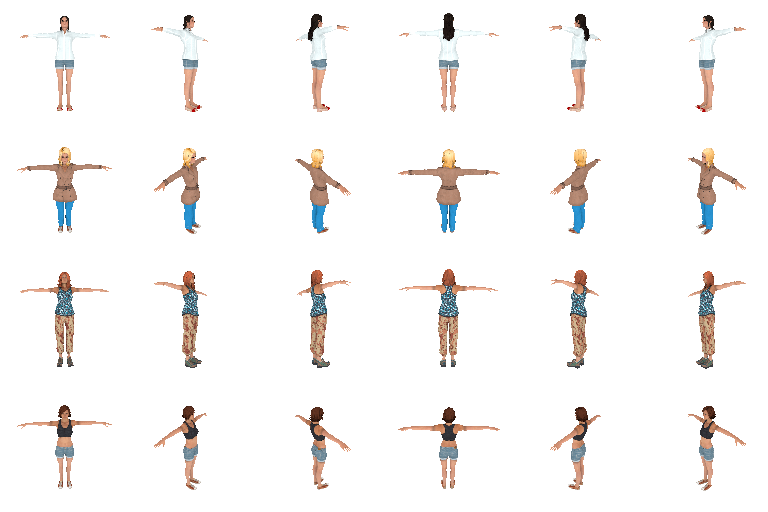
\includegraphics{data.png}
\caption{Synthetic Multiview Human Image Samples}
\end{figure}

We use a number of standard data augmentation techniques to preprocess our input data. We vary the lighting and camera position in Blender. We apply small random crops to the images, and randomly apply light Gaussian blur. Note that we do not perform random horizontal flips as we already have an image at the resulting view.

Since we use batch normalization \autocite{ioffe2015batch} for all layers, we do not normalize our input image. However, we do normalize the value of the target angle to [-0.5, 0.5] since it gets concatenated with the latent variables.

Since neural networks take a long time to train, all initial experiments are done using images of size 64x64. The final results are trained on images of 128x128 resolution. We notice significant improvements on the quality of our results when trained using higher resolution images, and we believe this improvement will continue as the resolution goes higher.

\section{Methods}

\subsection{Overview}

We tackle this problem using deep generative models. We divide our pipeline into two stages: the first stage consists of an input image, a target angle (0 to 360 degrees), and a conditional VAE. The encoder transforms the input image into a latent variable, concatenate it with the target angle, and passes them through the decoder. The decoded image should resemble the input image in the target angle, with noticeable artifact (e.g. blurry, sometimes with incorrect colors). The second stage consists of the original input image, output of the first stage (coarse image), and a conditional GAN. Both images are fed into a hierarchical feature extractor to obtain their latent representations. These latent representations are then concatenated and fed into a generator to obtain the final output. The generator is able to extract low level patterns from the original input image and generate a new image that conforms to the structure of the coarse image with patterns from the original input image.

Our network is written in Python using the Tensorflow framework. We trained our models using NVIDIA Tesla GPUs.

\begin{figure*}[htbp]
\centering
\includegraphics{Picture2.png}
\caption{Pipeline Overview}
\end{figure*}

\subsection{Stage 1: cVAE}

\begin{figure}[htbp]
\centering
\includegraphics{experiments.png}
\caption{Row 1-4: output of VAEs with (1) fully-connected layers only with insufficient amount of  hidden neurons (2) fully-connected layers only with sufficient hidden neurons (3) convolution layers with insufficient amount of filters (4) convolution layers with sufficient amount of filters. }
\end{figure}

We implemented the VAE from scratch, going from a simple fully-connected network with two hidden layers to a deep convolutional network consisting of 13 layers. Figure 4 shows the results of some of our intermediate work. Notice how the number of neurons is extremely important in capturing variation, and that convolution layers are much better at hierarchical representations.

The input is 128x128 pixels. The encoder consists of 6 convolution layers all with 3x3 kernels. The layers have 16, 16, 32, 32, 64, 1 filters respectively. We downsample the input twice with strided-convolutions. In the last layer, we flatten the result into a 1024-dimensional vector and pass it through a fully connected hidden layer to generate parameters to the learned distribution using the parameterization trick \autocite{kingma2013auto}. We use these parameters to sample our latent variables from a 400-dimensional Gaussian distribution and concatenate them with the normalized target angle. They then goes through a decoder that has a similar structure but in reverse, with two upsamples in the middle.

The loss function is defined as follows:

\begin{multline}
L(\theta;x, c)= -KL(q_\theta(z|x, c)||p(z|c))+ \\
E_{q_\theta(z|x, c)}[log(p_\theta(x|z, c))]
\end{multline}

\subsection{Stage 2: cGAN}

We attempted to implement a GAN from scratch. However, GAN is notoriously known for its instability and its difficulty to train. Our experience confirms this knowledge. Although the GAN community has proposed many techniques to make the training process easier \autocite{salimans2016improved, arjovsky2017wasserstein, karras2017progressive}, we decided not to implement one from scratch, but to build on top of an existing implementation \footnote{https://github.com/affinelayer/pix2pix-tensorflow}. There are several features of this implementation that we find desirable: it uses U-Net, which allows for better generation quality; it uses convolution transpose (fractionally-strided convolutions) instead of bilinear interpolation for upsampling; it uses Leaky ReLU instead of ReLU as activation functions. This implementation worked well without much hyperparameter tuning.

We modified the above implementation so that it takes two 128x128 sized images, passed them through an encoder with shared weights, concatenated their respective latent representations, and finally passed them through the decoder. We did not make any changes to the discriminator. The final generator is a 7-layer U-Net with 64, 128, 256, 512, 512, 512, 512 filters in each of the layers.

\section{Experimentation Results}

We use both quantitative and qualitative measures to assess the result of our work.

\subsection{Qualitative results}

The results of our final model is compared with other approaches and the ground truth (see Figure 5). Visually, our results have a more complete global appearance as well as more local details (note how the output of cGAN often loses patches of the body). At the same time, our result looks much sharper than the output of cVAE.

\begin{figure}[htbp]
\centering
\includegraphics{PICTURE4.png}
\caption{//TODO: change to image output summarize graph}
\end{figure}

\begin{figure}[htbp]
\centering
\includegraphics{samples.png}
\caption{Sample images trained and tested using synthetic images. Left to right: input image, output from cVAE, output from cGAN, our from our model, ground truth.}
\end{figure}

\subsection{Quantitative results}

For quantitative evaluation methods, we use Mean Square Errors (MSE), Structural Similarity Index (SSIM), and the Inception Score (IS) to compare the generated fine image output to target image, as a judgment for our model quality.

\begin{itemize}
\item Structural Similarity Index (SSIM) \autocite{wang2004image}: SSIM measures the similarity between two images. It's a better metric than the pixelwise error (MSE) as it insensitive to things like lighting conditions and small variation in poses. It's been used in other works on multiview synthesis \autocite{park2017transformation, zhao2017multi}. It's formally defined as:

$$SSIM(I_x,I_y)=\frac{(2\mu_x \mu_y + c_1)(2\sigma_{xy}+c_2)}{(\mu_x^2+\mu_y^2 +c_1)(\sigma_x^2+\sigma_y^2+c_2)}$$

\item Inception Score (IS): the Inception Score is adopted from Salimans' work on GANs \autocite{salimans2016improved} and is used to measure the quality of different generative models. The idea is that images that contain meaningful objects should have a conditional label distribution with low entropy while a model that generates varied images should have high entropy. The Inception Score is formally defined as:

$$IS(I_x, y)=exp(E_{I_x}D_{KL(p(y|I_x) || p(y))})$$
where $I_x$ is a generated image and $y$ is the label of that image predicted by the Inception model \autocite{szegedy2015going}.

\end{itemize}

For model comparison, we experimented the following 3 models on MVC and our synthetic dataset respectively, and compare their SSIM, IS, MSE measures:

\begin{itemize}
\item Using only cVAE.
\item Using only cGAN.
\item Using our VAE+GAN pipeline.
\end{itemize}

Figure 7 summarizes the result of our experimentations.
\begin{figure*}
  \includegraphics[width=\linewidth]{FigureTable.PNG}
  \caption{Experimental Results}
  \label{fig:boat1}
\end{figure*}

From the result metrics in the table, we can see that the following trends: 

\begin{itemize}
\item SSIM obtained by our VAE+GAN approach is larger than that of obtained by using VAE or GAN alone, which means our generated output image is more similar to the ground truth; 
\item IS score for VAE+GAN is larger than that of using VAE only, but smaller than IS score using GAN only, this is expected since GAN model alone allows more variation in the output images. 
\item MSE analysis shows that VAE+GAN MSE is smaller than that of using VAE or GAN alone, this resonates with the result of SSIM and proves that our approach in general has better performance generating images closer to target. 
\item In general, our model performs better on synthetic data than on real world data, this is because synthetic data is smoother, contains less details, and has similar pose, so the generation is relatively easier.
\end{itemize}

\section{Future Work}

Due to time constraints, there are many things on our roadmap that we haven't gotten to. Some of these things include:

\begin{itemize}
\item Improve the GAN: we only used a simple conditional GAN with very little hyperparameter tuning. There is a number of recently published papers that shows various techniques to improve the quality and stability of GANs.

\item Improve face synthesis: our model currently handles face poorly since it contains a lot of noticeable details. It is important to be able to recreate these details in a convincing way for good result. There are several promising attempts \autocite{yim2015rotating, huang2017beyond} that focuses solely on facial synthesis that we can follow up on.

\item Image background: our current dataset only contains images without any background. It is more difficult to synthesize views when the object of interest is not presented in isolation and we would like to tackle that problem in the future.

\item Transfer learning: we hope to use the model trained from our synthetic dataset on real images. Experiments on transfer learning \autocite{shrivastava2016learning} have shown great results for discriminative models. We hope to achieve similar results for generative models.
\end{itemize}

\section{Conclusion}
We aims at solving 360-degree full human body view synthesis problem by using our self-generated dataset and VAE+GAN modeling approach, while introducing some minor changes on modeling architecture and loss function compared with previous works [1,2,3].
Current preliminary results show some promising potential of our modeling approach. With the help of large volume self-generated human view data from 360 view angles, we hope we can solve the 360 degree full human body view synthesis problem and achieve state-of-art results.

\textbf{Teammate Contributions:}

Our teamwork break down:
\begin{itemize}
\item Si Wen: Si mainly worked on modeling, including VAE and variants of GAN modeling. He also contributed to the final report.
\item Tiancong Zhou: Tiancong mainly worked on the generation of our synthetic dataset and quantitative evaluation of our results.
\item Honghao Qiu: Honghao mainly worked on reporting and modeling. He is the main contributor to writing this report.
\end{itemize}

\printbibliography

\end{document}
